
\documentclass[11pt, titlepage, oneside, a4paper]{article}
\usepackage[T1]{fontenc}
\usepackage[utf8]{inputenc}
\usepackage[english]{babel}
\usepackage{amssymb, graphicx, fancyhdr}
\usepackage{listings}
\lstset{breaklines=true} 
\lstset{numbers=left, numberstyle=\scriptsize\ttfamily, numbersep=10pt, captionpos=b} 
\lstset{basicstyle=\small\ttfamily}
\newcommand{\inlineCode}{\lstinline[basicstyle=\normalsize\ttfamily]}
\addtolength{\textheight}{20mm}
\addtolength{\voffset}{-5mm}
\renewcommand{\sectionmark}[1]{\markleft{#1}}

% \Section ger mindre spillutrymme, använd dem om du vill
\newcommand{\Section}[1]{\section{#1}\vspace{-8pt}}
\newcommand{\Subsection}[1]{\vspace{-4pt}\subsection{#1}\vspace{-8pt}}
\newcommand{\Subsubsection}[1]{\vspace{-4pt}\subsubsection{#1}\vspace{-8pt}}
	
% appendices, \appitem och \appsubitem är för bilagor
\newcounter{appendixpage}

\newenvironment{appendices}{
	\setcounter{appendixpage}{\arabic{page}}
	\stepcounter{appendixpage}
}

\newcommand{\appitem}[2]{
	\stepcounter{section}
	\addtocontents{toc}{\protect\contentsline{section}{\numberline{\Alph{section}}#1}{\arabic{appendixpage}}}
	\addtocounter{appendixpage}{#2}
}

\newcommand{\appsubitem}[2]{
	\stepcounter{subsection}
	\addtocontents{toc}{\protect\contentsline{subsection}{\numberline{\Alph{section}.\arabic{subsection}}#1}{\arabic{appendixpage}}}
	\addtocounter{appendixpage}{#2}
}

% Ändra de rader som behöver ändras
\def\inst{Tillämpad fysik och elektronik}
\def\typeofdoc{Laborationsrapport}
\def\course{Script och webbrogrammering 7,5 hp}
\def\pretitle{Laboration 4}
\def\title{Python nr 2}
\def\name{Christer Jakobsson}
\def\username{dv12cjn}
\def\email{\username{}@cs.umu.se}
\def\graders{Ola Ågren, Kalle Prorok}



% Här brjar själva dokumentet
\begin{document}

	% Skapar framsidan (om den inte duger: gör helt enkelt en egen)
	\begin{titlepage}
		\thispagestyle{empty}
		\begin{large}
			\begin{tabular}{@{}p{\textwidth}@{}}
				\textbf{UMEÅ UNIVERSITET \hfill \today} \\
				\textbf{Institutionen för \inst} \\
				\textbf{\typeofdoc} \\
			\end{tabular}
		\end{large}
		\vspace{10mm}
		\begin{center}
			\LARGE{\pretitle} \\
			\huge{\textbf{\course}}\\
			\vspace{10mm}
			\LARGE{\title} \\
			\vspace{15mm}
			\begin{large}
				\begin{tabular}{ll}
					\textbf{Namn} & \name \\
					\textbf{E-mail} & \texttt{\email} \\
				\end{tabular}
			\end{large}
			\vfill
			\large{\textbf{Handledare}}\\
			\mbox{\large{\graders}}
		\end{center}
	\end{titlepage}


	% Fixar sidfot
	\lfoot{\footnotesize{\name, \email}}
	\rfoot{\footnotesize{\today}}
	\lhead{\sc\footnotesize\title}
	\rhead{\nouppercase{\sc\footnotesize\leftmark}}
	\pagestyle{fancy}
	\renewcommand{\headrulewidth}{0.2pt}
	\renewcommand{\footrulewidth}{0.2pt}

	
	
	\pagenumbering{arabic}

	% I Sverige har vi normalt inget indrag vid nytt stycke
	\setlength{\parindent}{0pt}
	% men däremot lite mellanrum
	\setlength{\parskip}{10pt}

	% Lägger in rubrik (finns \section, men då får man mycket spillutrymme)
	
	\Section{Del 1}
		\Subsection{Problembeskrivning}
		
		Detta python program skall fråga användaren om information om en bok användaren har läst och sedan skriva det till en fil som
		heter \emph{bibliotek.txt}. Den information som användaren skall ange är:
		\begin{itemize}
		\item Författare
		\item Titel
		\item Genre
		\item Genre2
		\item Datum när boken lästes
		\item Betyg i en skala, 1-5
		\item Egna kommentarer om boken
		\end{itemize}
		All information måste anges i rätt format och om användaren har matat in felaktig data till ett fält så upprepas frågan tills rätt format angetts.
		\Subsection{Algoritmbeskrivning}
		Fråga användaren om all information som
		ska föras in i filen. Användaren får mata in varje del tills dess att rätt format har angetts.
		
		Format på varje del:
		\begin{enumerate}
		\item[Författare] Får ej innehålla några siffror
		\item[Titel] Får innehålla tecken och siffror, måste vara en sträng.
		\item[Genre] Genre måste vara en av de tre fördefinierade titlarna som finns.
		\item[Genre2] Genre2 måste vara en av de fördefinierade subgenre's av den genre som valdes innan.
		\item[Datum läst] Måste vara i ett datum format (yy-mm-dd)
		\item[Betyg] Måste vara en siffra mellan 1-5
		\item[Kommentar] Får innehålla siffror och tecken, måste vara en sträng
		\end{enumerate}
		
		Efter att användaren har matat in rätt format i alla fält så öppnas filen \emph{bibliotek.txt} för skrivning och sedan skrivs en rad 
		med hela bokens information till filen, varje fält separerat med ett kommatecken[\emph{,}] och de fält som är strängar . 
		\Subsection{Exempelkörningar}
		\begin{itemize}
		 \item Körning 1: Korrekt indata
		 \subitem \begin{lstlisting}
lab4$ python del1.py 
Author: "TestAuthor"
Title: "TestTitle"
Genre: "Fiction"
Genre2: "Horror"
Type Date yy-mm-dd: 14-01-01
Grade (1-5): 1
Comments: "TestComments"
		\end{lstlisting}
		\item Körning 2: inkorrekt author
		 \subitem \begin{lstlisting}
lab4$ python del1.py 
Author: "test123"
Author cant contain digits, try again.
		\end{lstlisting}
		\item Körning 3: inkorrekt title
		 \subitem \begin{lstlisting}
lab4$ python del1.py 
Author: "Test"
Title: asd
Title should be text with surrounding "", ex: "Title".
Title:		
\end{lstlisting}
\item Körning 4: inkorrekt genre
		 \subitem \begin{lstlisting}
lab4$ python del1.py 
Author: "Test"
Title: "Test"
Genre: "Test"
Genre must be: ['Fiction', 'Fact book', 'Poetry']
\end{lstlisting}
\item Körning 5: inkorrekt genre2
		 \subitem \begin{lstlisting}
lab4$ python del1.py 
Author: "Test"
Title: "Test"
Genre: "Test"
Genre must be: ['Fiction', 'Fact book', 'Poetry']
Genre: "Fiction"
Genre2: "Test"
Genre2 must be: ['Detective', 'autobiograpyh', 'Horror', 'Comedy']
Genre2: 
\end{lstlisting}
\item Körning 5: inkorrekt datum
		 \subitem \begin{lstlisting}
lab4$ python del1.py 
Author: "Test"
Title: "Test"
Genre: "Fiction"
Genre2: "Horro"
Genre2 must be: ['Detective', 'autobiograpyh', 'Horror', 'Comedy']
Genre2: "Horror"
Type Date yy-mm-dd: 14 01 01
Wrong format, try again!
Type Date yy-mm-dd: 2014-01-01
Wrong format, try again!
Type Date yy-mm-dd: 
\end{lstlisting}
\item Körning 5: inkorrekt datum
		 \subitem \begin{lstlisting}
Grade (1-5): 0
Grade needs to be in range 1-5
Grade (1-5): 6
Grade needs to be in range 1-5
Grade (1-5): 
\end{lstlisting}
\item Körning 5: inkorrekt comments
		 \subitem \begin{lstlisting}
Comments: test
Comments should be text with surrounding "", ex: "Comments".
\end{lstlisting}

\end{itemize}

	\Section{Del 2}
		\Subsection{Problembeskrivning}
		Detta programs uppgift är att fråga användaren om en boktitel och sedan söka efter denna titel i \emph{bibliotek.txt} och om den hittas 
		skriva ut den raden. Programmet kan ta en titel när det har startats, eller ta flera titlar att söka efter som argument.
		\Subsection{Algoritmbeskrivning}
		Programmet frågar efter en boks titel och när denna har angetts så öppnas filen \emph{bibliotek.txt} för läsning.
		Sedan så läses datat in ifrån filen rad för rad och för varje rad så kollar programmet om titeln som eftersöktes stämmer med titeln på raden,
		om så är fallet så skrivs raden ut på stdout.
		För att skriva ut alla poster i filen så skriver man "ALL".
		\Subsection{Exempelkörningar}
		\begin{itemize}
		 \item Körning 1: Korrekt title
		 \subitem \begin{lstlisting}
lab4$ python del2.py 
Title To Search For (For all, type "ALL"): "TestTitle"
"TestAuthor", "TestTitle", "Fiction", "Horror", 2014-01-01, 1, "TestComments"
\end{lstlisting}
		 \item Körning 2: input som ej är en sträng
		 \subitem \begin{lstlisting}
lab4$ python del2.py 
Title To Search For (For all, type "ALL"): ejstrang
Error: input needs to be text with surrounding "", ex: "ALL".
Title To Search For (For all, type "ALL"): 
		\end{lstlisting}
		\item Körning 3: Sökt titel som inte finns
		 \subitem \begin{lstlisting}
lab4$ python del2.py
Title To Search For (For all, type "ALL"): "HEJ"
Title HEJ not found.
		\end{lstlisting}
		Kommentar: Om programmet inte hittar den titel det söker efter så skriver det ut det åpå standard error för att möjligheten att pipa eller 
		omdirigera output till en fil skall vara möjlig.
		\item Körning 4: Titlar som argument
		 \subitem \begin{lstlisting}
lab4$ python del2.py "asd" "TestTitle"
"asd", "asd", "Fact book", "Chemistry", 2014-01-01, 1, "No comments"
"TestAuthor", "TestTitle", "Fiction", "Horror", 2014-01-01, 1, "TestComments"
		\end{lstlisting}
		\end{itemize}
		
	\Section{Del 3}
		\Subsection{Problembeskrivning}
		Detta program skall implementera ett grafiskt gränssnitt som ska ha funktionaliteten ifrån de två programmen som beskrivits i 
		Del 1 och Del 2. Det ska alltså både innehålla en del där användaren kan lägga till en bok i filen och kan söka efter en boks titel och få 
		reda på all information om den titeln.
		
		\Subsection{Algoritmbeskrivning}
		Detta program ska binda samman de två tidigare delarna och implementera dessa i ett grafiskt gränssnitt. 
		Därmed har den underliggande koden i princip samma algoritmbeskrivning som föregående delar förutom att
		det är kopplat till ett grafiskt gränssnitt som ska vara så tydligt, enkelt och intuitivt att använda som möjligt.
		\Subsection{Exempelkörningar}
		\begin{itemize}
		 \item Körning 1: Add Data
    \subitem \begin{figure}[h]
    \centering
    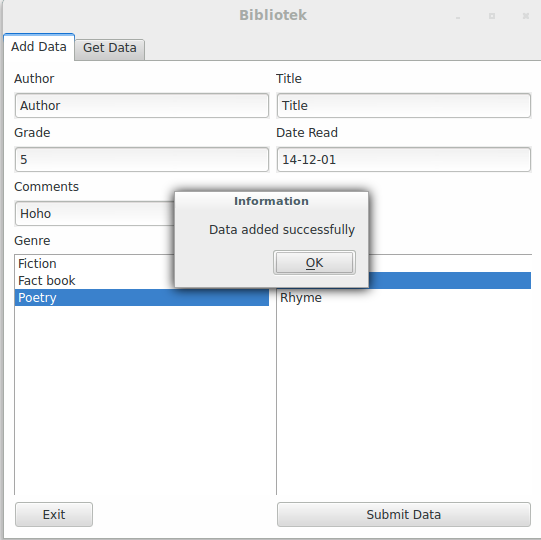
\includegraphics[width=0.7\textwidth]{successAdd.png}
    \caption{Add Data}
    \label{fig:succesAdd}
\end{figure}

Kommentar: Har matat in korrekta värden i alla fält och sedan tryckt på \emph{Submit Data}.
	\newpage
	\item Körning 2: Fält ej ifyllt korrekt: Exempel där datum inte är ifyllt korrekt
    \subitem \begin{figure}[h]
    \centering
    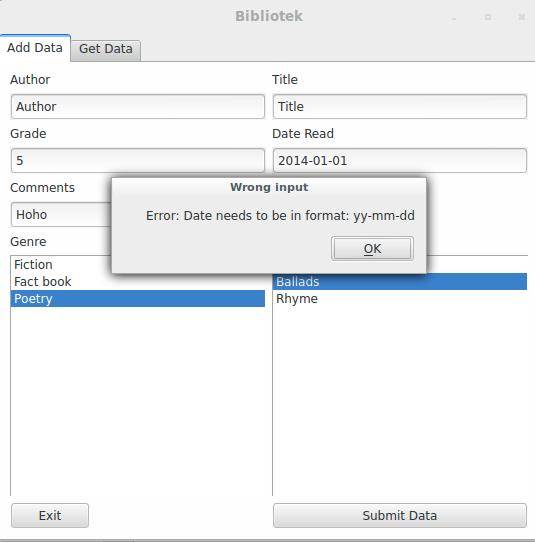
\includegraphics[width=0.7\textwidth]{datumFail.png}
    \caption{Fel input	}
    \label{fig:Wrong input}
\end{figure}

Kommentar: Har matat in korrekta värden i alla fält förutom i datumfältet och sedan tryckt på \emph{Submit Data}, datat läggs inte in och användaren 
får ett felmeddelande.

  \newpage
 
    \item Körning 3: Get data
    \subitem \begin{figure}[h]
    \centering
    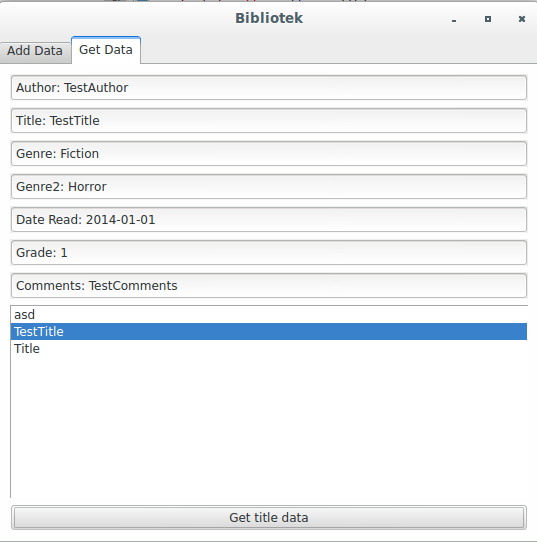
\includegraphics[width=0.7\textwidth]{getSuccess.png}
    \caption{Get Data}
    \label{fig:getData}
\end{figure}

Kommentar: Har valt titeln \emph{TestTitle} och sedan klickat på \emph{Get title data}, Datat visas i fälten ovanför listan.
		\end{itemize}

	\Section{Del 4}	
		\Subsection{Problembeskrivning}
		Denna del skall innehålla två stycken program, ett program som ska vara en klient med ett gui som ser ut och har samma funktionalitet som föregående del. 
		Men som inte ska skriva och läsa direkt ifrån filen \emph{bibliotek.txt} utan ska kommunicera med den andra delen som skall vara en server som skall sköta all skrivning
		och läsning ifrån filen.
		Kommunikationen ska ske genom sockets så att klienten och servern inte behöver ligga på samma dator.
		\Subsection{Algoritmbeskrivning}
		När klienten skickar till server så skickar den ett kommando följt av ett mellanslag sedan eventuell data som server behöver, Ex \emph{[GET\_ALL\_DATA]} 
		de kommandon som klienten och server använder sig av är:
		
		\newpage
		\begin{itemize}
		 \item GET\_ALL\_DATA
		 \subitem Klienten skickar detta meddelande till servern när den vill få ut information om alla böcker som finns i filen.
		 \item GET\_TITLE\_DATA \emph{Boktitel}
		 \subitem Dette meddelande skickar klienten när den vill få all information om en specifik titel ifrån servern.
		 \item SEND\_ROW\_DATA \emph{Bokdata}
		 \subitem Används när klienten vill lägga in en ny bok i biblioteket.
		\end{itemize}

		\Subsubsection{Klient}
		För att användaren ska kunna lägga till eller hämta data ifrån servern måste användaren ansluta till servern.
	        Därefter så kan användaren lägga till böcker via \emph{Add tab} eller hämta en boks data via \emph{Get data} tabben.
	        
	        \emph{Add Data}: 
	        \begin{itemize}
	         \item Användaren får skriva in värden i varje fält, Author, Title etc
	         \item Användaren trycker på \emph{Submit Data}, om alla fält har korrekt input
	         \subitem Öppna filen för skrivning och skriv raden med bokens information till slutet på filen
	         \subitem Stäng filen, En popup som meddelar användaren att det gick bra visas.
	         \item Om något fält inte är korrekt ifyllt kommer en popup visas och meddela användaren vilket fält som är fel.
	        \end{itemize}
	        
	        \emph{Get data}
	        \begin{itemize}
	         \item Användaren får klicka på den boktitel den vill ha all information ifrån.
	         \item När användaren har valt en titel och klickar på \emph{Get title data} 
		 \subitem Filen öppnas för läsning, den eftersökta titelns bokrad söks efter
		 \subitem När boktiteln hittas så fylls fälten i med information från bokens alla poster.
		 \item Filen stängs och användaren ser bokens information i textfälten.
	        \end{itemize}


		\Subsubsection{Server}
		Add data:
		\begin{itemize}
		 \item Servern får kommandot [SEND\_ROW\_DATA \emph{Bokdata}]
		 \item Plockar ut \emph{Bokdata} och lagrar det i en datastruktur
		 \item Skriver datat till filen, stänger filen och skickar ett ok till klienten att det gick bra.
		\end{itemize}

		Get all data:
		\begin{itemize}
		 \item Servern får ett kommando [GET\_ALL\_DATA] ifrån klienten
		 \item Öppnar filen för läsning, läser in alla poster ifrån filen och skickar det till klienten.
		\end{itemize}
		
		Get row data:
		\begin{itemize}
		 \item Servern får ett kommando [GET\_ROW\_DATA \emph{Boktitel}]
		 \item Öppnar filen för läsning
		 \item Söker efter raden med den titeln
		 \item Stänger filen och returnerar titels data till klienten
		\end{itemize}

		\Subsection{Exempelkörningar}
		Exempelkörningarna kommer att se likadana ut i denna del som i Del 3, i och med att denna dels klient ser likadan ut som
		i del 3. Servern har inget grafiskt gränssnitt men den har utskrifter när den tar emot ett kommando och när den skickar 
		data till klienten.
		
		\newpage
				\begin{itemize}
		 \item Körning 1: Ansluta till servern. 
    \subitem \begin{figure}[h]
    \centering
    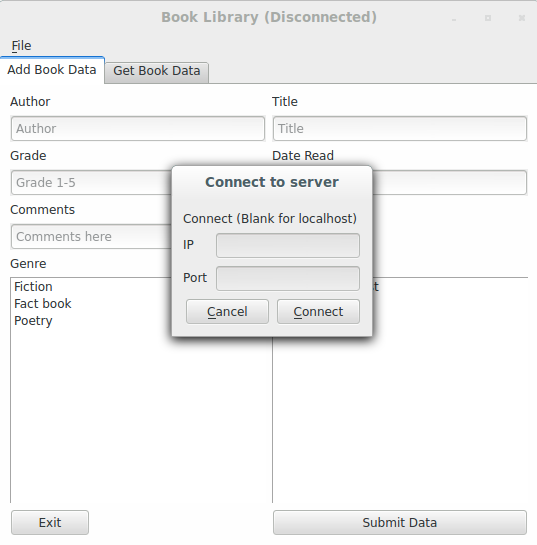
\includegraphics[width=0.7\textwidth]{connectToServer.png}
    \caption{Anslutning till server}
    \label{fig:connect}
\end{figure}
\newpage
\begin{figure}[h]
    \centering
    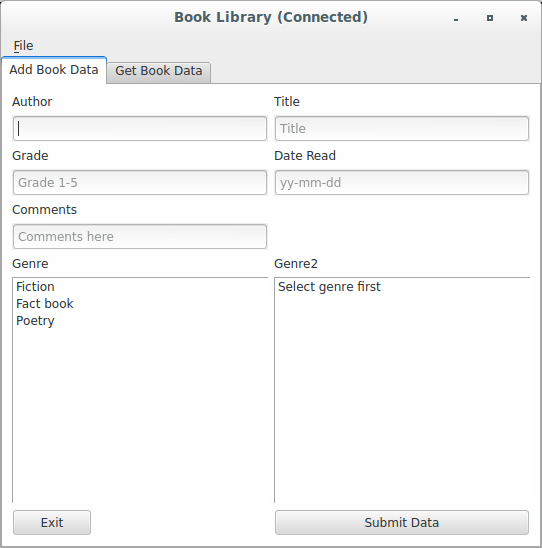
\includegraphics[width=0.7\textwidth]{connectServerSuccess.png}
    \caption{Anslutning lyckats}
    \label{fig:connectServerSuccess}
\end{figure}

\begin{lstlisting}
lab4$ python server.py 
Socket now listening (Exit server with CTRL+C)
Server: got connection from client 127.0.0.1:34447
\end{lstlisting}


Kommentar: Den första bilden \ref{fig:connect} visar hur programmet ser ut vid start, användaren upmanas att skriva in en server att ansluta till, eller lämna blank om server
ligger på den lokala datorn. Bild \ref{fig:connectSuccess} visar hur hur programmet ser ut vid en lyckad anslutning, notera (Connected) uppe i fönstrets list.
Koden visar hur serversidan ser ut när användaren lyckats anslutit.

    \item Körning 2: Add Data
    \subitem \begin{lstlisting}
[SEND\_ROW\_DATA]
127.0.0.1:34447 sends SEND\_ROW\_DATA
Sending 200 OK
Server: got connection from client 127.0.0.1:34447
             \end{lstlisting}
		 \item Körning 3: Refresh List

    \begin{lstlisting}
[GET\_ALL\_DATA]
127.0.0.1:34447 sends GET\_ALL\_DATA
sending reply
Server: got connection from client 127.0.0.1:34447
             \end{lstlisting}

Kommentar: I del 3:s lösning så uppdateras listan med bokdata automatiskt när programmet startar, men i en server/klient lösning så kan det vara bra att skicka så lite
data emellan servern och klienten som möjligt. Därför måste klienten klicka på \emph{Refresh List} för att skicka en förfrågan till servern på av få all data.
	
			 \item Körning 4: Get Row Data

    \begin{lstlisting}
[GET\_TITLE\_DATA]
127.0.0.1:35171 sends GET\_TITLE\_DATA
Title [TestTitle]
Sending reply
Server: got connection from client 127.0.0.1:35171
             \end{lstlisting}
             
Kommentar: Titlen som efterfrågas av klienten är \emph{TestTitle}
\end{itemize}

\end{document}